\section{指针}
{\large``我认为赋值语句和指针变量可以说是计算机科学最具价值的宝藏。''\footnote{原文:I do consider assignment statements and pointer variables to be among computer science's ``most valuable treasures.''}}
\begin{flushright}——高德纳\footnote{高德纳(Donald Ervin Knuth),美国计算机科学家和数学家,1974年图灵奖得主。高德纳成就颇丰,其中最负盛名的是它的著作《计算机程序设计艺术》(\textit{The Art of Computer Programming})。}\end{flushright}
\subsection*{内存与地址}
在一个C/C++程序运行时,内存中会存储着有关这个程序的信息。我们可以把这些内存空间分为五个区段(如图5.1所示):
\begin{itemize}
    \item 代码段(Code/Text Section)。这个区域存储着一系列指令,可以告诉电脑这个程序要做什么。比如说,函数的定义就在在代码区中,这部分内容告诉电脑它要做什么。
    \item 数据段(Data Section)。这个数据区不意味着``存储所有的数据''。它只存储一些全局变量或已初始化的静态变量,也就是在函数之外的域中定义的数据\footnote{我们会在第七章讲解有关知识。}
    \item BSS段(BSS Sectino)。通常用于存放未初始化的静态变量。
    \item 栈段(Stack Section)。局部变量(比如主函数中定义的变量)和每次函数调用时的实参等信息,都存储在栈区(想想我们上一章中讲到的``调用栈'')。每次我们定义一个新数据,这个数据的信息就会被压入栈中,当这个数据的作用域结束时,它就会出栈。
    \item 堆段(Heap Section)。用于动态内存分配。我们会在本章中介绍动态内存分配。
\end{itemize}
\begin{figure}[htbp]
    \centering
    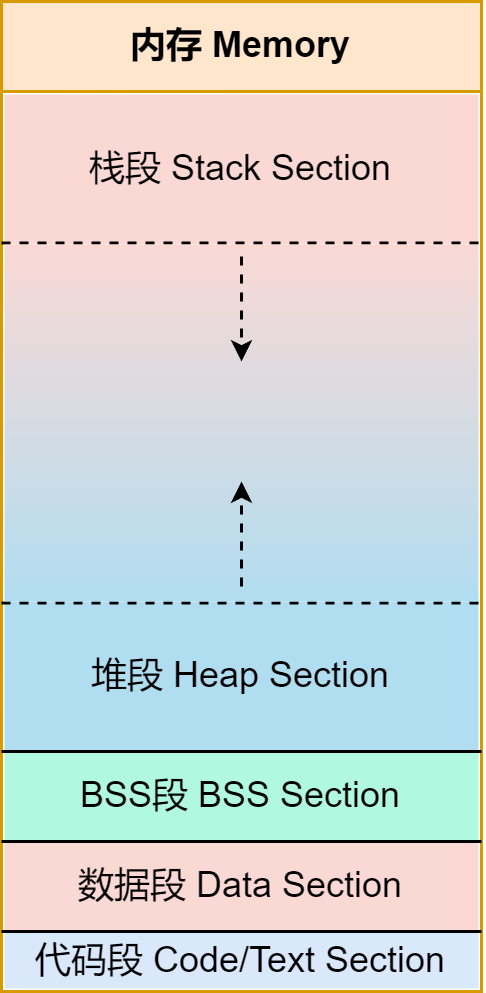
\includegraphics[width=0.25\textwidth]{../images/generalized_parts/05_layout_of_memory_300.png}
    \caption{程序的内存布局}
\end{figure}\par
内存中有无数字节,不同的数据需要不同的字节数量来存储,我们可以用 \lstinline@sizeof@ 来计算字节数量的值。\par
既然内存中有这么多字节,那么程序要怎么判断自己要用的数据在哪里呢?这就需要用到\textbf{内存地址(Memory address)}了。\par
内存中的每个字节都有一个内存地址。就像我们根据门牌楼号来找到一间房子那样,程序也需要通过内存地址才能快速找到一个字节,并且读取或者修改它的值。\par
举例来说,我们在主函数中定义一个 \lstinline@char@ 型变量,命名为 \lstinline@ch@。在运行时,每当遇到了这个指令,程序就会在栈段当中找到一个闲置的字节,用来存储这个变量的值。那假如我们定义一个 \lstinline@double@ 型的变量 \lstinline@d@ 呢?程序会在栈区中找到八个连续的闲置字节(在绝大部分系统中,\lstinline@double@ 型的内存空间占用都是8字节),用来存储这个变量的值。\par
在C++中,\lstinline@&@ 运算符可以对某个变量求地址。一般说来,如果要输出地址的话,地址值都是用十六进制的形式\footnote{即,以 \lstinline@0x@ 开头(有些编译环境,如MSVC,输出的地址值是不带 \lstinline@0x@ 开头的,所以别惊讶),后面表示为 \lstinline@0@\~{}\lstinline@F@(或用小写)的一串数字,如 \lstinline@0xe23df5cc@。}来表示的。\lstinline@&@ 运算符单独作用于一个变量时,返回值是它的地址\footnote{并不是所有的数据都可以取地址!我们会在精讲篇中说明,它关系到左值和右值的问题。}。
\begin{lstlisting}
int main() {
    double d {3.1415926}; //定义一个double型变量d
    cout << &d; //用&取d的地址值并输出
}
\end{lstlisting}
这个程序的输出结果是:\\\noindent\rule{\linewidth}{0.2pt}\texttt{
0x7ffccff275b8
}\\\noindent\rule{\linewidth}{0.2pt}
不同计算机的实际情况可能大相径庭,不同编译器处理内存分配的方式也可以大同小异,所以这个地址的具体值因机器而异,我们需要在意的只是格式。在这里,它输出了一个十六进制的结果,这正是 \lstinline@d@ 的地址值。\par
细心的读者可能会有疑问:\lstinline@d@ 作为一个 \lstinline@double@ 型数据,明明占据了八个字节,为什么输出结果只给了我们一个地址呢?\par
这是因为,对于任何一种类型,在取地址时\textbf{只会返回它的第一个字节的地址}。因为任何一个变量占据的内存都是连续的一段,所以我们只要知道了第一个字节在哪里,当然就知道整个变量占据了哪个区间的内存了。\par
\begin{figure}[htbp]
    \centering
    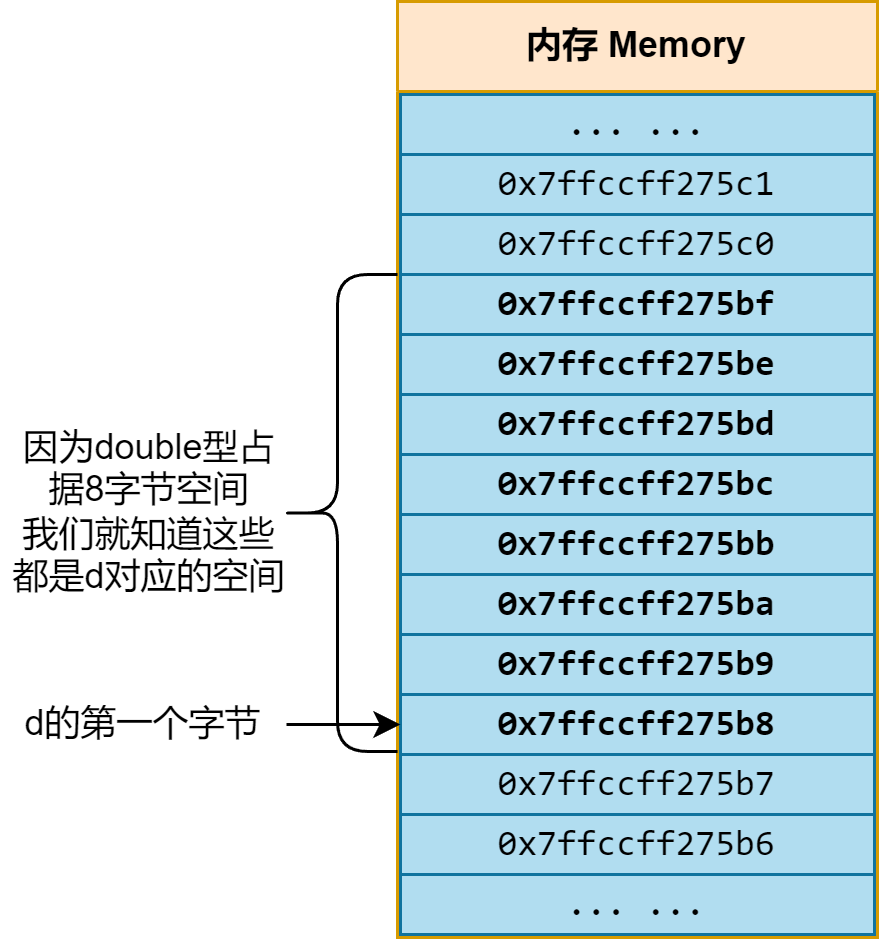
\includegraphics[width=0.6\textwidth]{../images/generalized_parts/05_address_of_types_in_memory_300.png}
    \caption{\lstinline@d@ 在内存空间中的示意图}
\end{figure}
如图5.2所示,既然 \lstinline@0x7ffccff275b8@ 是 \lstinline@d@ 的地址,而 \lstinline@sizeof(double)@ 又是 \lstinline@8@,那么自然而然,\lstinline@d@ 的信息应当存储在从 \lstinline@0x7ffccff275b8@ 开始的8个字节,一直到 \lstinline@0x7ffccff275bf@ 为止。\par
\textbf{所以无论哪个类型,其内存地址指的都是它所占内存空间中的第一个字节的地址\footnote{除非你重载了取地址函数 \lstinline@&@,这种情况我们不讨论。}。}请牢记这点,它会让你后面的学习过程更轻松的。\par
补充一条:读者可能会在自己尝试的时候发现一个有趣的现象:如果试图输出一个 \lstinline@char@ 类型的地址,输出的结果可能会是各种奇奇怪怪的内容,但绝对不像是个指针。我们会在字符串那一节再介绍这个问题。如果你坚定地想输出 \lstinline@char@ 变量的地址,你可以采用这种写法:
\begin{lstlisting}
    char ch {48}; //定义char型变量并赋初值'0'
    cout << (void*)&a; //指针类型转换为void*,这样就会以地址值的形式输出
    // 也可以把(void*)&a换作reinterpret_cast<void*>(&a)
\end{lstlisting}
\subsection*{指针的定义和使用}
仅仅知道地址值还不够,我们很难把它用起来。我们的当务之急是,找到一种可以``存储地址值''的数据类型。可是很遗憾,虽然地址值的表示方式像一个整数,但是我们不能把它的值存到整型数据当中。实际上,C/C++专门有一大类存储地址值的数据类型,叫作\textbf{指针变量},简称\textbf{指针(Pointer)}。\par
请留意,\textbf{指针不是一个数据类型,而是``一群''数据类型}。``指向\lstinline@int@ 的指针''和``指向 \lstinline@double@ 的指针''是不同的数据类型。\par
定义一个指针的基本语法如下,这里有两种主流写法可供选择,它们是等价的:
\begin{lstlisting}
    <类型>* <指针名>; //*写在<类型>一侧,与<指针名>分开
    <类型> *<指针名>; //*写在<指针名>一侧,与<类型>分开
\end{lstlisting}\par
第一种写法更清晰,它说明了这个名字是一个指针类型。
\begin{lstlisting}
    int a {0}; //定义一个int型变量a,并初始化为0
    int* pa {&a}; //定义一个int指针pa,并初始化为a的地址
\end{lstlisting}
但是它也会引发一些困惑……
\begin{lstlisting}
    int* p1, p2; //p1是int*类型,但p2是int类型!没想到吧
\end{lstlisting}\par
第二种写法则不会出现这种困惑,因为本身就是要在指针名一侧写 \lstinline@*@ 的。
\begin{lstlisting}
    int *p_1, p_2, *p_3; //p_1和p_3是int*类型,而p_2是int类型
\end{lstlisting}
这种写法还能降低其它有关问题的理解成本,我们很快就会遇到。\par
那么究竟使用哪种写法呢?不同的人当然有不同的理解和习惯,不必强求。不过在编写本书的过程中,我选择我最喜欢的写法:只在描述返回类型的时候用第一种写法,否则用第二种写法。\par
习惯上,我们喜欢把``\lstinline@p@ 存储了 \lstinline@a@ 的地址''称为``\lstinline@p@ 指向了 \lstinline@a@''。这当然是一种很形象的表述,但很多教材会为了这点``形象''而忽略了对本质的阐述,这是得不偿失的。\par
现在让我们假想这样一个过程:我先定义了一个 \lstinline@double@ 型的变量 \lstinline@d@,然后又定义了一个 \lstinline@double*@ 型的变量 \lstinline@pd@(这是一个指针变量)。
\begin{lstlisting}
    double d {3.14159}; //定义一个double型变量d
    double *pd {&d}; //定义一个double*型指针变量pd,它指向d
\end{lstlisting}
理论上讲,一个程序只要知道了某个变量的地址,就具备了读取或修改对应内存空间的能力。那么 \lstinline@d@ 这个名字,也就无所谓有没有了。我们能否只根据 \lstinline@pd@ 中保存的地址值,就实现读取和修改 \lstinline@d@ 的功能呢?当然可以!\par
这里我们需要一个运算符:取内容运算符 \lstinline@*@\footnote{也有很多资料将其称为解引用运算符。}。读者可能会困惑——这不是乘法运算符吗?其实你可以把它当作一种重载!当它接收两个操作数时,它的含义就是乘法运算;当它接收一个操作数时,它的含义就是取指针的内容(见图5.3)。\par
\begin{figure}[htbp]
    \centering
    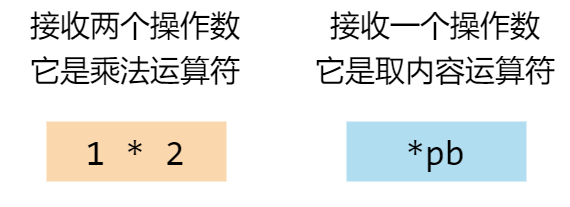
\includegraphics[width=0.45\textwidth]{../images/generalized_parts/05_operator_dereference_or_multiplication_300.png}
    \caption{我们可以把 \lstinline@*@ 接收不同数量操作数的情况当成一种重载}
\end{figure}
说回原来的话题。通过 \lstinline@*@ 运算符,我们可以无需变量名就可以读取一个指针的内容;而且在允许的情况下,我们还可以修改其内容,这个修改是直接对内存中的内容进行修改,和修改 \lstinline@d@ 的值一样直截了当。\par
\begin{lstlisting}
    double d {3.14159}; //定义一个double型变量d
    double *pd {&d}; //定义一个double*型指针变量pd,它指向d
    cout << *pd << endl; //输出pd取内容的结果,当然是3.14159
    *pd = 2.71828; //修改pd对应内存中的内容,等效于直接修改d的值
    cout << d; //输出d的值,会发现结果是2.71828
\end{lstlisting}
读者可以自行运行这段程序,或者写一些别的代码试试,会发现 \lstinline@d@ 和 \lstinline@*pd@ 的特征非常相似,它们几乎就是同一个事物!\par
从本质上讲,变量的名字只是一个``表象''而已,藏在背后的最关键的东西还是内存中对应的若干字节中存储的信息。C/C++允许我们自定义变量名,这样的好处在于,我们可以不必像汇编语言那样,用一些枯燥的 \lstinline@rip@, \lstinline@rsp@, \lstinline@eax@ 之类的名字来描述真实世界中丰富多彩的信息,而是用一些顾名思义的名词,让我们和别人看了都能懂。\par
但计算机还是要把这些名字还原成内存中的一个个信息,然后再处理。变量名对于计算机来说,只是一个绑定了相应内存地址的名字罢了。于是 \lstinline@d@ 和 \lstinline@*pd@ 没什么分别;\lstinline@&d@ 和 \lstinline@pd@ 也没什么分别。图5.4阐述了它们的关系。\par
\begin{figure}[htbp]
    \centering
    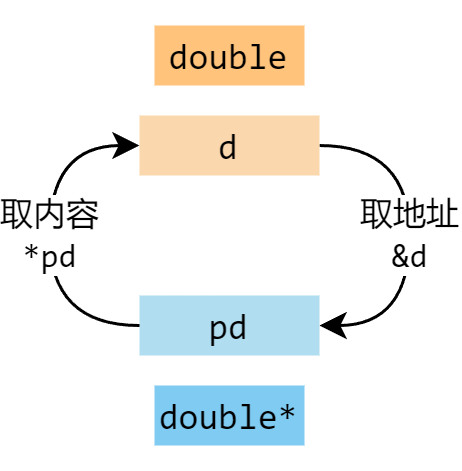
\includegraphics[width=0.4\textwidth]{../images/generalized_parts/05_relationship_between_variables_and_pointers_300.png}
    \caption{变量 \lstinline@d@、地址 \lstinline@&d@、指针 \lstinline@pd@ 与内容\lstinline@*pd@ 的相互关系}
\end{figure}
这个关系是循环的,我们可以先取地址再取内容,最后得到的东西和 \lstinline@d@ 是一回事。所以我们还可以对这个东西再取地址,再取内容,再取地址,再取内容……以至无穷。
\begin{lstlisting}
    cout << *&*&*&d; //*&*&*&d相当于*&*&d,相当于*&d,相当于d
\end{lstlisting}
不过这种写法就太没意义了,绕了一大圈,最后还是回到 \lstinline@d@。实际编程中我们不会这么做。\par
但是不要止步于此。指针的存在还为我们提供了一种新的可能性:我们可以绕过``变量名''这一步,直接用指针来访问和修改内存中的信息。这是我们后续要讲的指针参数传递、数组和动态内存分配的基础。\par
\subsection*{指针参数传递}
在写函数的时候,我们可能会试图通过函数来改变实参的值。举个例子,我们想写一个函数 \lstinline@exchange@,来交换它的两个实参的值。为了方便阐述,我在这里就不用函数模版了,我们假定它接收两个 \lstinline@int@ 参数。
\begin{lstlisting}
void exchange(int a, int b) { //这里只需实现副作用,无需求值,故设返回类型void
    int tmp {a}; //定义一个临时变量tmp,用以存储a的值
    a = b; //赋值,现在a获得了b的值,我们的目标完成一半
    b = tmp; //赋值,现在b获得了tmp的值,也就是a原来的值
    return ; //对于返回类型为void的函数来说,return是可有可无的
}
int main() {
    int a {3}, b {4}; //定义a=3,b=4
    exchange(3, 4); //交换a和b的值,预期是a变成4,b变成3
    cout << a << ' ' << b; //输出a和b的值,检验一下
    return 0;
}
\end{lstlisting}
这个程序的运行结果是\\\noindent\rule{\linewidth}{0.2pt}\texttt{
3 4
}\\\noindent\rule{\linewidth}{0.2pt}
这个代码的逻辑看上去很正确,但是为什么它完全不起作用呢?\par